%% ===========================================
%% Nation-wise Failure Distribution
%% Version 4 - Fixed overlapping issues
%% ===========================================

\documentclass[tikz,border=3pt]{standalone}
\usepackage{tikz}
\usepackage{pgfplots}
\pgfplotsset{compat=1.18}
\usetikzlibrary{calc, positioning, arrows.meta, decorations.pathreplacing}

% Colorblind-safe palette (Okabe-Ito based)
\definecolor{c_nonlatin}{RGB}{230,159,0}    % orange
\definecolor{c_ocr}{RGB}{86,180,233}        % sky blue
\definecolor{c_math}{RGB}{204,121,167}      % reddish purple
\definecolor{c_reason}{RGB}{0,114,178}      % strong blue
\definecolor{c_other}{RGB}{180,180,180}     % neutral gray

\begin{document}

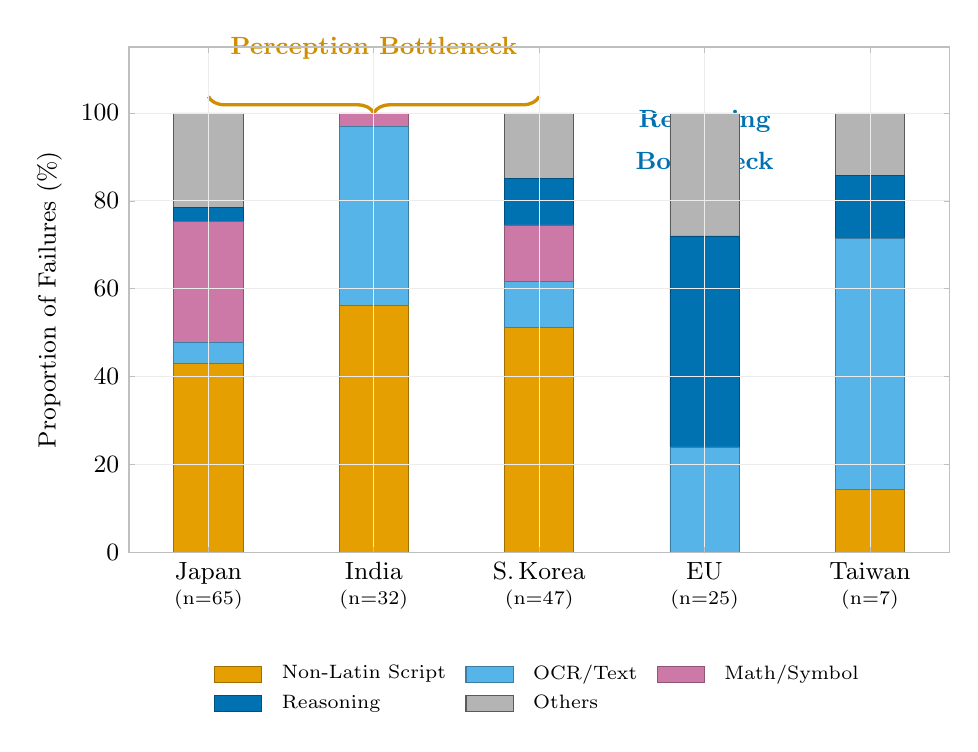
\begin{tikzpicture}
\begin{axis}[
    ybar stacked,
    bar width=25pt,
    width=12cm,
    height=8cm,
    ylabel={Proportion of Failures (\%)},
    ymin=0,
    ymax=115,
    ytick={0,20,40,60,80,100},
    xtick=data,
    symbolic x coords={Japan, India, S.Korea, EU, Taiwan},
    xticklabels={
        {Japan\\[-2pt]{\scriptsize(n=65)}},
        {India\\[-2pt]{\scriptsize(n=32)}},
        {S.\,Korea\\[-2pt]{\scriptsize(n=47)}},
        {EU\\[-2pt]{\scriptsize(n=25)}},
        {Taiwan\\[-2pt]{\scriptsize(n=7)}}
    },
    xticklabel style={align=center, font=\small},
    y tick label style={font=\small},
    ylabel style={font=\small},
    legend style={
        at={(0.5,-0.20)},
        anchor=north,
        legend columns=3,
        font=\scriptsize,
        column sep=5pt,
        draw=none,
    },
    legend cell align={left},
    enlarge x limits=0.12,
    clip=false,
    axis on top,
    grid=major,
    major grid style={gray!15, line width=0.3pt},
    axis line style={gray!50},
    tick style={gray!50},
    major tick length=2pt,
]

% Non-Latin Script (orange)
\addplot+[
    ybar stacked,
    fill=c_nonlatin,
    draw=c_nonlatin!70!black,
    line width=0.3pt,
    forget plot,
] coordinates {
    (Japan, 43.1)
    (India, 56.3)
    (S.Korea, 51.1)
    (EU, 0)
    (Taiwan, 14.3)
};

% OCR/Text Recognition (sky blue)
\addplot+[
    ybar stacked,
    fill=c_ocr,
    draw=c_ocr!70!black,
    line width=0.3pt,
    forget plot,
] coordinates {
    (Japan, 4.6)
    (India, 40.6)
    (S.Korea, 10.6)
    (EU, 24.0)
    (Taiwan, 57.1)
};

% Math/Symbol (reddish purple)
\addplot+[
    ybar stacked,
    fill=c_math,
    draw=c_math!70!black,
    line width=0.3pt,
    forget plot,
] coordinates {
    (Japan, 27.7)
    (India, 3.1)
    (S.Korea, 12.8)
    (EU, 0)
    (Taiwan, 0)
};

% Pure Reasoning (strong blue)
\addplot+[
    ybar stacked,
    fill=c_reason,
    draw=c_reason!70!black,
    line width=0.3pt,
    forget plot,
] coordinates {
    (Japan, 3.1)
    (India, 0)
    (S.Korea, 10.6)
    (EU, 48.0)
    (Taiwan, 14.3)
};

% Others (neutral gray)
\addplot+[
    ybar stacked,
    fill=c_other,
    draw=c_other!50!black,
    line width=0.3pt,
    forget plot,
] coordinates {
    (Japan, 21.5)
    (India, 0)
    (S.Korea, 14.9)
    (EU, 28.0)
    (Taiwan, 14.3)
};

% Manual legend
\addlegendimage{area legend, fill=c_nonlatin, draw=c_nonlatin!70!black}
\addlegendentry{Non-Latin Script}
\addlegendimage{area legend, fill=c_ocr, draw=c_ocr!70!black}
\addlegendentry{OCR/Text}
\addlegendimage{area legend, fill=c_math, draw=c_math!70!black}
\addlegendentry{Math/Symbol}
\addlegendimage{area legend, fill=c_reason, draw=c_reason!70!black}
\addlegendentry{Reasoning}
\addlegendimage{area legend, fill=c_other, draw=c_other!50!black}
\addlegendentry{Others}

% ===== Key percentage labels (positioned carefully) =====

% Japan: Non-Latin 43% - center of orange segment (0 to 43.1)
\node[font=\scriptsize\bfseries, text=black] at (axis cs:Japan, 22) {43\%};

% India: Non-Latin 56% - center of orange segment (0 to 56.3)
\node[font=\scriptsize\bfseries, text=black] at (axis cs:India, 28) {56\%};
% India: OCR 41% - center of sky blue segment (56.3 to 96.9)
\node[font=\scriptsize\bfseries, text=black] at (axis cs:India, 77) {41\%};

% S.Korea: Non-Latin 51% - center of orange segment (0 to 51.1)
\node[font=\scriptsize\bfseries, text=black] at (axis cs:S.Korea, 26) {51\%};

% EU: Reasoning 48% - center of blue segment (24 to 72)
\node[font=\scriptsize\bfseries, text=white] at (axis cs:EU, 48) {48\%};

% ===== Bottleneck annotations =====

% Perception Bottleneck brace above Japan to S.Korea
\draw[decorate, decoration={brace, amplitude=6pt, mirror, raise=2pt}, 
      very thick, c_nonlatin!90!black]
    (axis cs:Japan, 105) -- (axis cs:S.Korea, 105);
\node[font=\small\bfseries, c_nonlatin!90!black, above=8pt] 
    at (axis cs:India, 105) {Perception Bottleneck};

% Reasoning Bottleneck label for EU with arrow
\draw[-{Stealth[length=5pt, width=4pt]}, line width=1pt, c_reason]
    (axis cs:EU, 90) -- (axis cs:EU, 74);
\node[font=\small\bfseries, c_reason, above=2pt] 
    at (axis cs:EU, 92) {Reasoning};
\node[font=\small\bfseries, c_reason, below=-2pt] 
    at (axis cs:EU, 92) {Bottleneck};

\end{axis}
\end{tikzpicture}

\end{document}
